

%%%%%%%%%%%%%%%%%%%%%%%%%%%%%%%%%%%%%%%%%
% Academic Title Page
% LaTeX Template
% Version 2.0 (17/7/17)
%
% This template was downloaded from:
% http://www.LaTeXTemplates.com
%
% Original author:
% WikiBooks (LaTeX - Title Creation) with modifications by:
% Vel (vel@latextemplates.com)
%
% License:
% CC BY-NC-SA 3.0 (http://creativecommons.org/licenses/by-nc-sa/3.0/)
% 
% Instructions for using this template:
% This title page is capable of being compiled as is. This is not useful for 
% including it in another document. To do this, you have two options: 
%
% 1) Copy/paste everything between \begin{document} and \end{document} 
% starting at \begin{titlepage} and paste this into another LaTeX file where you 
% want your title page.
% OR
% 2) Remove everything outside the \begin{titlepage} and \end{titlepage}, rename
% this file and move it to the same directory as the LaTeX file you wish to add it to. 
% Then add \input{./<new filename>.tex} to your LaTeX file where you want your
% title page.
%
%%%%%%%%%%%%%%%%%%%%%%%%%%%%%%%%%%%%%%%%%

%----------------------------------------------------------------------------------------
%	PACKAGES AND OTHER DOCUMENT CONFIGURATIONShttps://www.overleaf.com/project/5f9756abfb48e8000183dcde
%----------------------------------------------------------------------------------------

\documentclass[11pt]{article}

%%Packages

\usepackage{appendix}

%Matematiske
\usepackage{amsmath} %Blant annet referer til likninger
\usepackage{amsfonts} %Inneholder matematiske fonter mathbb
\usepackage{physics}


%Grafisk
\usepackage{graphicx}
\usepackage{subcaption}
\usepackage{float} %Brukes med H for å sette posisjon til figur
\usepackage{pythonhighlight}
\usepackage{listings}
\usepackage{xcolor} % for setting colors
\usepackage{setspace}

%Kommentar
\usepackage[colorinlistoftodos]{todonotes}

%Til hyperlinker
\usepackage[colorlinks=true, breaklinks]{hyperref}%Breaklink deler opp linken dersom for lang

\usepackage[utf8]{inputenc} % Required for inputting international characters
\usepackage[T1]{fontenc} % Output font encoding for international characters

\usepackage{baskervillef} % Palatino font

% kode
\usepackage[ruled,vlined]{algorithm2e}
\lstset { %
	language=C++,
	backgroundcolor=\color{black!5}, % set backgroundcolor
	basicstyle=\footnotesize,% basic font setting
}
\usepackage[top=2.5cm, bottom=2.5cm, left=2.5cm, right=2.5cm]{geometry}
\parindent = 0cm


\begin{document}
	%----------------------------------------------------------------------------------------
	%	TITLE PAGE
	%----------------------------------------------------------------------------------------
	
	\begin{titlepage} % Suppresses displaying the page number on the title page and the subsequent page counts as page 1
		\newcommand{\HRule}{\rule{\linewidth}{0.5mm}} % Defines a new command for horizontal lines, change thickness here
		
		\center % Centre everything on the page
		
		%------------------------------------------------
		%	Headings
		%------------------------------------------------
		
		\textsc{\LARGE University of Oslo}\\[1.5cm] % Main heading such as the name of your university/college
		
		\textsc{\Large FYS3150}\\[0.5cm] % Major heading such as course name
		
		\textsc{\large Computational Physics}\\[0.5cm] % Minor heading such as course title
		
		%------------------------------------------------
		%	Title
		%------------------------------------------------
		
		\HRule\\[0.4cm]
		
		{\huge\bfseries The Ising Model for Magnetic Materials\\
		\Large{Modelling Magnetic Phase Transitions Devising the\\ Metropolis - Hastings Algorithm}\\[0.4cm] % Title of your document
		}
		\HRule\\[1.5cm]
		
		%------------------------------------------------
		%	Author(s)
		%------------------------------------------------
		
		%	\begin{minipage}{0.4\textwidth}
		%		\begin{flushleft}
		%			\large
		%			\textit{Author}\\
		%			B.J. \textsc{Blazkowicz} % Your name
		%		\end{flushleft}
		%	\end{minipage}
		%	~
		%	\begin{minipage}{0.4\textwidth}
		%		\begin{flushright}
		%			\large
		%			\textit{Supervisor}\\
		%			Dr. Caroline \textsc{Becker} % Supervisor's name
		%		\end{flushright}
		%	\end{minipage}
		
		% If you don't want a supervisor, uncomment the two lines below and comment the code above
		{\large\textit{Authors}}\\
		\textsc{Lars Kristian Skaar}\\
		\textsc{Håkon Lindholm}\\
		\textsc{Brage Brevig} % Your name
		\\
		\url{https://github.uio.no/lkskaar/FYS3150}
		%------------------------------------------------
		%	Date
		%------------------------------------------------
		
		\vfill\vfill\vfill % Position the date 3/4 down the remaining page
		
		{\large\today} % Date, change the \today to a set date if you want to be precise
		
		%------------------------------------------------
		%	Logo
		%------------------------------------------------
		
		\vfill\vfill
		%
\includegraphics[width=0.5\textwidth]{logouio.png}\\[6cm] % Include a department/university logo - this will require the graphicx package
		
		%----------------------------------------------------------------------------------------
		
		%\vfill % Push the date up 1/4 of the remaining page
		
	\end{titlepage}

	%---------------------------------------------------------------------------------%-------
	\newpage
	\setstretch{1.5}
	\setlength\parindent{0pt}
	
	\section{Abstract}
    The Markov Chain Monte Carlo (MCMC) - based Metropolis - Hastings Algorithm (MHA) is here devised to study two - dimensional spin lattices, herein via the Ising model. The study has a ladder - like structure, in which we first study the simple 2x2 spin lattice in order to compare our numerical implementation of the MHA against benchmark analytical solutions. Having studied the performance of our program, we proceed to explore the larger 20x20 spin lattice from which we are able to determine the MCMC equilibration time, which we use to optimize the random sampling of even larger spin lattices. The physical systems, regardless of size, are studied in detail by considering aspects such as energy distribution, expectation values for quantities such as energy and absolute magnetization, and lastly the critical temperature $T_C$. We find that our implementation of the MHA produces numerical results which commit relatives error of order $10^{-5}$ for 10$^{6}$ Monte Carlo sweeps through the 2x2 lattice, and that the larger 20x20 spin lattice reaches a steady state within the range of 5$\cdot10^{3}$ - 10$^{4}$ Monte Carlo sweeps when the spin lattice is initially disordered. The study of even larger systems lead to results which clearly indicate configurational phase transitions, which in turn allowed us to numerically extract the critical temperature in an infinitely large spin lattice. We found this to hold the value of $2.289$, deviating from the theoretical value obtained by Onsager ($T_C = 2/\sqrt{1 + \sqrt{2}} \approx 2.269)$ by 0.8\%. 
	
	
	
	\newpage
	\tableofcontents
	\newpage
	
	\section{Introduction}
Just short of one year ago, the world first learnt of the Covid-19 virus, which has since then gone on to change the everyday life of people all around the globe. The family of coronaviruses (CoV) have been identified many times before, causing illnesses which may manifest themselves somewhere between the common cold and more severe disease. The introduction of a novel virus, however, calls for detailed studies of how different social and medical measures, alongside seasonal variation and vital dynamics have an impact on the short - and long term development of the number of infected agents within a network. The wording we devise in this article is deliberate, as this model does not only apply to human beings in a larger population, but also to other entities such as biological cells, or other non-sentient nodes in networks in which we may, as an example, study the communicable flow of information.
This study is designed to develop a numerical model for the spread of contagious disease in a network of agents. To do this, we work via the SIRS\footnote{Susceptible - Infected - Recovered - Susceptible} model and implement it numerically first through a set of coupled ordinary differential equations (ODEs), and later by a stochastic model in order to also capture the random nature of reality in our simulations. The stochastic modelling is in itself an interesting study, as the model may be applied in different areas of research such as information, rumor and substance addiction dynamics in a network. We will first go into detail on the SIR(S) model and its underlying assumptions, before we move on to explain how it may be numerically implemented, whether it is deterministically or stochastically. We shall then present select findings from our studies, and discuss them in light of both the numerical implementation and the effects of adding several layers of realism such as seasonal variation in rate of contagion and vaccination measures. Lastly, we make some summary remarks on the presented work.
\newpage
	\section{Theory \& Background}

\subsection{Mathematical Background}
Consider a set of lattice sites $\mathcal{L}$, each with its own set of adjacent lattice sites forming an $n$-dimensional lattice. For each lattice site $\ell \in \mathcal{L}$ there exists a discrete variable $s_\ell$ wherein $s_\ell \in \{+1,-1\}$. These discrete values numerically represent the orientation of the spin at site $\ell$ either being $\uparrow (+1)$, or $\downarrow (-1)$. We take $s_i = (s_\ell)_{\ell\in\mathcal{L}}$ to be the spin configuration at lattice site $\ell$, and $s$ to be the net spin configuration of the entire spin - lattice. Two adjacent sites $\ell_1, \ell_2 \in \mathcal{L}$ are coupled through an spin - spin interaction of magnitude $J_{\ell_1,\ell_2}$. In the most general formulation of this problem, one should also assume that at each site $\ell$, the spin is coupled to an external magnetic field $\mathcal{H}_\ell$. The Hamiltonian describing a specific spin configuration $s$ for a spin - lattice containing $N$ spin sites is then given by
\begin{equation}
    E^{(s)} = H(s) = -\sum_{\langle ij \rangle}^{N}J_{ij}s_is_j - \mu \sum_{j}^{N}\mathcal{H}_js_j
    \label{mostgeneralhamiltonian}
\end{equation}
where $E^{(s)}$ should be read as the energy of a specific spin configuration $s$. Here $\langle ij \rangle$ is a short hand indication of $i$ and $j$ being closest neighbors in the lattice, and $\mu$ denotes the magnetic moment. In this study we shall assume that the spin - lattices are not under the influence of an external magnetic field, such that $\mathcal{H}_j = 0,\ \ \forall\ j \in N$. We also assume that the interaction between any two spins is the same for all spin pairs such that $J_{ij} = J,\ \ \forall\ \langle ij \rangle \ \in \mathcal{L}$. In summary, we are therefore concerned with spin configurations $s$ whose energies are 
\begin{equation}
    E^{(s)} = H(s) = -J\sum_{\langle ij \rangle}^{N} s_is_j
    \label{specifichamiltonian}
\end{equation}
The sign in equation \eqref{specifichamiltonian} is conventional, and commits the following properties for different signs of $J$; if $J > 0$, the spins are in ferromagnetic order, if $J < 0$ the spins are in antiferromagnetic order and if $J \equiv 0$, the spins are noninteracting. In this study, we take $J > 0$, and by that we are studying ferromagnetic spin - spin interactions. Next to the energy of particular spin configurations, we are also interested in the net magnetization $M^{(s)}$ arising from the alignment of all spins in a spin - lattice. This is simply the sum of all assigned spin - values at all sites $i$ in a given spin - lattice
\begin{equation}
    M^{(s)} = \sum_{i}^{N}s_i
    \label{magnetization}
\end{equation}
where $M^{(s)}$ should be read as the magnetization of a given spin configuration $s$. For macroscopic spin systems, the different spin configurations are distributed with a probability according to the Boltzmann distribution
\begin{equation}
    P(s) = \frac{e^{-\beta E^{(s)}}}{Z_\beta}
    \label{boltzmann}
\end{equation}
with $\beta = 1/k_B T $ where $k_B$ is Boltzmann's constant, and $T$ is the absolute temperature of the spin system measured in Kelvin. $Z_\beta$ is known as a partition function where 
\begin{equation}
    Z_\beta = \sum_s e^{-\beta E^{(s)}}
    \label{partitionfunc}
\end{equation}
acting as a normalization constant, describing the system at thermodynamical equilibrium.\\

As we are dealing with microstates whose existence are probabilistically distributed according to equation \eqref{boltzmann}, it follows that physical observables attributed to this system behave accordingly, meaning that there are certain energies, or magnetic configurations which are more likely to find, id est expected values. Generally, the expectation value of any function $f(s)_\beta$ varying with the spin configuration $s$ at a fixed $\beta$ (fixed temperature $T$) may be computed through
\begin{equation}
    \langle f \rangle_\beta = \sum_{s}f(s)P(s)
\end{equation}
such that the expectation value of the energy of this system is
\[
\langle E \rangle = \frac{1}{Z_\beta}\sum_{s}E^{(s)}e^{-\beta E^{(s)}} = -\frac{\partial}{\partial \beta}\ln Z_\beta
\]
Similarly, the expectation value of the absolute magnetization of the system is
\[
\langle |M| \rangle = \frac{1}{Z_\beta}\sum_{s}|M^{(s)}|e^{-\beta E^{(s)}}
\]


\subsection{Benchmark Example; a 2x2 Ising Model}
Designing efficient and precise scientific software is often hinged on being able to compare numerical results against analytical ones, where they exist. The most discerning reality one must face in the Ising model, is that the partition function $Z_\beta$ will quickly become close to impossible to determine analytically for large numbers of spins $N$, as the number of possible configurations follow $2^N$. Luckily, low-dimensional spin - lattice systems have analytical expressions for many of the physical attributes we are interested in studying. We shall therefore study a simple 2x2 Ising model, before going on to study larger two-dimensional systems. It will be our business to study the expected energy, $\langle E \rangle$, and absolute magnetization, $\langle |M| \rangle$, of a given system, as well as the heat capacity at constant volume, $C_V$, and magnetic susceptibility $\mathcal{X}$.\\

Our goal now is to arrive at analytical expression for the different physical observables we are interested in studying, as to use them as yardsticks against which we may compare our numerical results. We need to launch off into this section by first undergoing the task of determining the partition function $Z_\beta$ for a 2x2 spin - lattice. 


\begin{figure}[h]
	\centering
	\begin{subfigure}{0.45\linewidth}
	\centering
	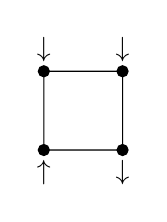
\begin{tikzpicture}
	\filldraw 	(0,0) circle(2pt) node[align=left, below]{$\uparrow$}-- 
				(0,1) circle(2pt) node[align=left, above]{$\downarrow$}-- 
				(1,1) circle(2pt) node[align=right, above]{$\downarrow$}-- 
				(1,0) circle(2pt) node[align=right, below]{$\downarrow$}-- (0,0);
	\end{tikzpicture}
	\caption{}
	\label{fig:4folddegen2by2lattice}
	\end{subfigure}
    \begin{subfigure}{0.45\linewidth}
    \centering
    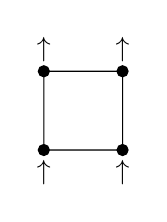
\begin{tikzpicture}
	\filldraw 	(0,0) circle(2pt) node[align=left, below]{$\uparrow$}-- 
				(0,1) circle(2pt) node[align=left, above]{$\uparrow$}-- 
				(1,1) circle(2pt) node[align=right, above]{$\uparrow$}-- 
				(1,0) circle(2pt) node[align=right, below]{$\uparrow$}-- (0,0);
	\end{tikzpicture}
	\caption{}
	\label{fig:2by2lattice}
    \end{subfigure}
    \caption{Simple 2x2 spin lattices with four - fold degeneracy (a), and single - fold degeneracy (b).}
\end{figure}
Consider Figure \ref{fig:4folddegen2by2lattice}, representing one of sixteen possible spin configurations in this system. This specific configuration has no net energy, which may be calculated through equation \eqref{specifichamiltonian}. Observe, however, that changing the position of the lonesome spin-up ($\uparrow$) to any of the other three corners of the lattice does not change the energy of the system - any configuration containing one spin up and three spin down is what we call a \textit{degenerate} configuration. In this case, the configuration is four - fold degenerate, which we choose to denote by $\mathcal{D}(s) = 4$. The magnetization of this particular configuration is $M = -2$, which may be calculated by equation \eqref{magnetization}. Such consideration need to be made for all sixteen possible spin configurations in the 2x2 spin lattice, and are summarized in the table below
\begin{table}[h!]
    \centering
    \caption{Tabular overview of associated degeneracies, energies and magnetizations for different spin - up configurations.}
    \begin{tabular}{c|c|c|c|c}
         \hline 
         Number of spin - up & $\mathcal{D}(s)$ & $E^{(s)}$ & $M^{(s)}$ & $|M|^{(s)}$ \\
         \hline
         4 & 1 & -$8J$ & 4 & 4\\
         3 & 4 & 0 & 2 & 2\\
         2 & 4 & 0 & 0 & 0\\
         2 & 2 & $8J$ & 0 & 0\\
         1 & 4 & 0 & -2 & 2\\
         0 & 1 & -$8J$ & -4 & 4\\
         \hline
    \end{tabular}
    
    \label{tab:latticevals}
\end{table}

Using the tabulated values in Table \ref{tab:latticevals}, and inserting them into equation \eqref{partitionfunc}, we arrive at
\begin{equation}
    Z_\beta = 2e^{8J\beta} + 2e^{-8J\beta} + 12 = 4\cosh(8J\beta) + 12
\end{equation}
Having established a closed form solution of $Z_\beta$, we may now unpack useful closed form solution of $\langle E \rangle$, $\langle |M| \rangle$, $C_V$ and $\mathcal{X}$ as functions of $\beta = 1/k_BT$. The expectation value of the energy as a function of $\beta$ becomes
\begin{equation}
    \langle E \rangle_\beta = -\frac{\partial}{\partial \beta}\ln Z_\beta = -8J\frac{\sinh(8J\beta)}{\cosh(8J\beta) + 3}
    \label{Energyclosedform}
\end{equation}
The heat capacity of the system at constant volume, $C_V$, correlates the energy variance at a temperature, to temperature it self through 
\[
C_V = \frac{1}{k_B T^2}\sigma^2_E = \frac{1}{k_B T^2}\left(\langle E^2 \rangle_\beta - \langle E \rangle^2_\beta\right)
\]
We may observe that the last term in the equation above is equivalent to
\begin{equation}
    C_V = \frac{1}{k_B T^2}\frac{\partial}{\partial \beta}\langle E \rangle _ \beta = \frac{192J^2}{k_B T^2}\frac{\cosh(8J\beta)}{\left(\cosh(8J\beta) + 3\right)^2}
    \label{heatcap}
\end{equation}
Moving on to the expected absolute magnetization, we may establish a closed form solution of this quantity by inserting values from Table \ref{tab:latticevals} into equation \eqref{magnetization}. This leads to
\begin{equation}
    \langle |M| \rangle_\beta = \frac{1}{Z_\beta}\left(8e^{8J\beta} + 16\right) = \frac{4\left(2e^{8J\beta} + 4\right)}{4\left(\cosh(8J\beta) + 3\right)} = \frac{2e^{8J\beta} + 4}{\cosh(8J\beta) + 3}
    \label{mabs}
\end{equation}
Observe simultaneously that 
\[
\langle M^2 \rangle_\beta = \frac{1}{Z_\beta}\left(32e^{8J\beta} + 32\right) = \frac{8e^{8J\beta} + 8}{\cosh(8J\beta) + 3}
\]
Together, these two expressions are related to the magnetic susceptibility $\mathcal{X}_\beta$ of the system through
\begin{equation}
    \mathcal{X}_\beta = \frac{1}{k_B T}\sigma^2_M = \frac{1}{k_B T}\left(\langle M^2 \rangle_\beta - \langle |M| \rangle^2_\beta \right) = \frac{1}{k_B T} \frac{\left(8e^{8J\beta}+8\right)\left(\cosh(8J\beta) + 3\right) - \left(2e^{8J\beta} + 4\right)^2}{\left(\cosh(8J\beta) + 3\right)^2}
    \label{suscept}
\end{equation}
At this point, we are able to determine analytical values for all of the physical quantities we may study in the 2x2 Ising model for a given temperature $T$. This allows us to study the performance of our algorithm closely, as we shall see in the Results section. 

\subsection{Critital Temperature, $T_C$}\label{sectioncritical}
In real materials, the number of particles (which would carry the spin-attribute) quickly becomes incredibly vast. A gram of solid material usually contains a number of particles within range of Avogadro's number ($\sim 10^{23}$), which puts the execution of the MHA not only at risk of overflow, but also gives computation times no ordinary student has the time, or willpower, to endure. The second-order phase transition we study in this project is characterized by a correlation length which spans the whole system. Since we are always limited, and severely so, to a finite lattice, we can devise so called finite size scaling relations, relating the behaviour of finite lattices with the results of infinitely large lattices. The critical temperature then scales as
\begin{align}
    T_C(\mathcal{L}) - T_C(\mathcal{L} = \infty) &= a\mathcal{L}^{-1/\nu}\label{critical}
\end{align}
The analytical value for the critical temperature was found by Lars Onsager \cite{statphys} to be approximately $2.269$ K.\\ \\
By setting $\nu = 1$, we can rewrite \eqref{critical} as
\begin{align}
    T_C(\mathcal{L}) &= a\mathcal{L}^{-1} + T_C(\mathcal{L}=\infty)\label{critical2}
\end{align}
This is a linear equation with the intercept as the critical temperature for an infinite lattice. We can then extract the critical temperature for several lattice sizes, and find the intercept by linear regression to approximate the analytical value. 
	\section{Numerical Methods \& Implementation}
\subsection{Markov Chains and Random Walks}
Consider a one dimensional finite point lattice where we start at a random position $x$. At each time step, we make a jump. Either one step to the left, or one step to the right.
The initial position is $x = j\Delta x$, where $\Delta x$ is the length of each jump. Whether we jump left or right, our next position will be $x = i\Delta x$. A probability distribution function (PDF) of the points on the lattice is given by $w_i(t)$, where $i$ is the specific position on the lattice. We also define a transition probability matrix, $W(j\rightarrow i)$. The time development of the system with the PDF and transition probability matrix is now given by
\begin{align}
    w_i(t) &= \sum_jW(j\rightarrow i)w_j(t)\label{markovknown}
\end{align}
When the transition probability matrix is known, \eqref{markovknown} will give us the steady state of the system when we allow $t\rightarrow \infty$.
\begin{equation*}
\lim_{t \rightarrow \infty} \abs{\omega(t + \delta) - \omega(t)} = 0
\end{equation*}
The fact that this time development is only dependent on the previous step is a key feature of Markov Chains that is very suitable for the Ising model. We can now implement this in our program by only using the previous state.

From this we get the eigenvalue equation with eigenvalue $\lambda = 1$:
\begin{equation}
    W \omega(t = \infty) = \omega(t = \infty)
\end{equation}
We can now use this to create a way of transitioning from one state to another. Assuming $W \  \in \ \ \mathbb{R}^{n x n}$ with eigenvectors $\{ v_1, v_2, ... , v_n \}$. We can then write the next state as 
\begin{eqnarray*}
\omega_0 &=& \sum^n_{i=1}a_iv_i \\
\omega_1 &=& \sum^n_{i=1} \lambda_i a_iv_i\\
&\vdots& \\
\omega_m &=& \sum^n_{i=1}\lambda_i^m a_i v_i
\end{eqnarray*}
with $a$ as an unknown coefficient. The problem we now encounter is the fact that the transition matrix $W$ is either unknown or too complicated to calculate. 

\subsection{The Metropolis Algorithm}
In our case, the transition probability matrix $W(j\rightarrow i)$ is not known to us. We therefore model it as a product of two probabilities
\begin{align}
    W(j\rightarrow i) &= T(j\rightarrow i)A(j\rightarrow i)
\end{align}
where $T(j\rightarrow i)$ is the probability for making a transition from a state $j$ to a state $i$, and $A(j\rightarrow i)$ is the probability of accepting a proposed move from state $j$ to state $i$. The time development of the system can then be expressed as
\begin{align}
    w_i(t+1) &= \sum_j\left[w_j(t)T_{j\rightarrow i}A_{j\rightarrow i} + w_i(t)T_{i\rightarrow j}(1-A_{i\rightarrow j})\right]\label{transition}
\end{align}
if we assume that $T$ and $A$ are time-independent. Since all probabilities are normalized, we can use that $\sum_jT_{i\rightarrow i} = 1$, to rewrite \eqref{transition} to
\begin{align}
    w_i(t+1) - w_i(t) &= \sum_j\left[w_j(t)T_{j\rightarrow i}A_{j\rightarrow i} - w_i(t)T_{i\rightarrow j}A_{i\rightarrow j}\right]
\end{align}
When $t\rightarrow \infty$ we require that that $w_i(t+1) = w_i$ such that
\begin{align}
    \sum_jw_jT_{j\rightarrow i}A_{j\rightarrow i} &= \sum_jw_iT_{i\rightarrow j}A_{i\rightarrow j}
\end{align}
To avoid generating cyclic solutions, we introduce a condition, namely a detailed balance
\begin{align}
    W(j\rightarrow i)w_j &= W(i\rightarrow j)w_i\\
    \frac{w_i}{w_j} = \frac{W(j\rightarrow i)}{W(i\rightarrow j)} &= \frac{T_{j\rightarrow i}A_{j\rightarrow i}}{T_{i\rightarrow j}A_{i\rightarrow j}}
\end{align}
For the Ising model, we use the Boltzmann distribution as our PDF, such that
\begin{align}
    w_i &= \frac{e^{-\beta(E_i)}}{Z}
\end{align}
which states the probability of finding the system in a state $i$ with the energy $E_i$, when $\beta = 1/k_BT$. Z is a partition function. This now gives us
\begin{align}
    \frac{w_i}{w_j} &= e^{-\beta(E_i - E_j)} = e^{-\beta\Delta E} = \frac{T_{j\rightarrow i}A_{j\rightarrow i}}{T_{i\rightarrow j}A_{i\rightarrow j}}
\end{align}
Since the partition function is cancelled out, we never need to worry about it at all. The most simple form of the Metropolis algorithm, is called the \textit{brute force Metropolis algorithm}, which is the algorithm employed in this project. The brute force algorithm assumes that $T_{i\rightarrow j}$ is symmetric, meaning that $T_{i\rightarrow j} = T_{j\rightarrow i}$. This leads to
\begin{align}
    \frac{A_{ij}}{A_{ji}} &= e^{-\beta\Delta E}
\end{align}
The expression above means that lower energy states are most probable. If we were to accept only moves to states of lower energy, the results of our algorithm would be biased and give a wrong representation of the random walk process. We therefore must allow moves to states of higher probability, and define the acceptance probability $A_{ij}$ as
\begin{align}
    A_{ij} &=
    \begin{cases}
    e^{-\beta\Delta E}, \qquad \text{for }\Delta E > 0\\
    1, \qquad\qquad\,\, \text{else}
    \end{cases}\label{cases}
\end{align}
which means that if a move to a state of lower energy is proposed, we accept the move, meaning that $A_{ij} = 1$. If a move to a higher state of energy is proposed, we must check the acceptance probability $A_{ij}$ with the ratio between the probabilities from our PDF. \\ \\
We have now laid the mathematical ground work for the \textit{brute force Metropolis algorithm} following numerical recipe\\

\fbox{\parbox{\textwidth}{Brute Force Metropolis - Hastings Algorithm:
\begin{enumerate} \item Initialize a spin lattice with $\mathcal{L}$ spins on its two axes, with a corresponding energy $E_i$ and absolute magnetization $|M_i|$. The initial configuration may be chosen to be ordered or disordered. 
\item Use a random number generator to seed a random site in the lattice. Propose then a new configuration by forcing a spin flip on the seeded site.
\item Calculate $\Delta E$ with the seeded site as a local spin center using periodic boundary conditions.
\begin{itemize}
    \item If $\Delta E \leq 0$, accept the new configuration.
    \item If $\Delta E > 0$, calculate $w = e^{-\beta\Delta E}$ and compare with a random number $\in [0,1]$. If the random number is less or equal to $w$, accept the proposed transition in configuration space. Otherwise, reject it.
\end{itemize}
\item Update the expectation values.
\item Repeat for a given amount of Monte Carlo cycles.\end{enumerate}}}\\

After we've gone through the desired number of Monte Carlo cycles, the expectation values may be normalized by dividing by the number of Monte Carlo Cycles. Here, we also divide the expectation value by the total number of spins in the lattice as to obtain the expectation values per spin.\\ \\
The Ising model has a huge advantage that will help us massively in our calculations. It turns out that $\Delta E$ can only take on 5 possible values! Since we limit ourselves to flipping one spin at a time, we need only concern ourselves with the four nearest neighbors, following the expression for the Hamiltonian of Ising systems.
\begin{figure}[H]
    \centering
    \includegraphics[width = 0.7\linewidth]{Figure/figur1.png}
    \caption{For a spin up center, these are the five possible combinations of the neighboring spins, and their accompanying energy before and after the center spin is flipped.}
    \label{fig:deltae}
\end{figure}
Figure \ref{fig:deltae} shows the five possible changes in energy that can occur when flipping the spin at one point. From the figure, we see that these changes in energy are $\Delta E = \{8J, 4J, 0, -4J, -8J\}$. Since for all non zero values of $\Delta E$ there also an equal, negative $\Delta E$, these five possible outcomes also holds for a spin down center lattice point. This means that we can pre-calculate these values, and do not have to evaluate the change in energy for every MCS, which tremendously lowers the computational cost.

\subsection{Implementation}
\subsubsection{Periodic boundary conditions}
When calculating the energy of the system in a specific configuration $i$, we employ so-called \textit{periodic boundary conditions}. For a one dimensional lattice of length $\mathcal{L}$, with particles $s_1, s_2,..,s_L$, this means that the neighbor to the left of $s_1$ takes the value of $s_L$, and the neighbor to the right of $s_L$ takes the value of $s_1$. This is implemented in the following way\\ \\
\begin{algorithm}[H]
		\caption{Periodic boundary conditions}
		\label{periodic}
		\SetAlgoLined
		\SetKwFunction{Fperiodic}{periodicBoundaryCondition}
		\Fperiodic{$i$, $dimension$, $variable$}{\\
		    \quad (i+dimension+variable) \% dimension\;
		\KwRet\;
		}
\end{algorithm}

This simple little function will return the index of the nearest neighbor to an input lattice point $i$, depending on whether the neighbor is to the left or above, $variable = -1$, or to the right or below, $variable = +1$. This costs us 3 FLOPs, if we consider the modulus operator to count as 1 FLOP. For the neighbor to the left of $s_1$, which is at index $(0)$, the function will return the numerical value of \textit{dimension}, which equals $\mathcal{L}$, the dimension of the lattice. \\ \\
A more efficient way to implement these boundary conditions would be to initialize the lattice with dimension $\mathcal{L} + 2$, where the extra two lattice points would contain the value of the last lattice point on the other side of the lattice. This means that when initializing, we would give the first value, $s_1$ to the second lattice index, $(1)$, and also to the last lattice index, $(\mathcal{L}+1)$. This would be done in a similar way for all other end points. When our program updates $s_1$, it would also update $s_{L+2}$. This would free us from having to call the function in Algorithm \ref{periodic}, four times for every computation of $\Delta E$, which would save us 12$\mathcal{L}^2$ FLOPs\footnote{Floating Point Operations.} per Monte Carlo sweep.

% Ikke helt sikker på denne seksjonen
\subsection{Units}
As was mentioned in the Theory \& Background Section, the coupling constant $J$ and the Boltzmann constant $k_B$ are both set to one in our simulation, that is $J = k_B = 1$. This kind of natural constant scaling is implemented as to avoid under - or overflow errors in our computations, as these constants may take on very numerical values which are difficult to represent accurately on a 64-bit computer. 


	\section{Results}

\begin{table}[H]
\centering
\caption{Run times for MC method and RK4 method with 10$^5$ integration points and 30 stochastic simulations}
\begin{tabular}{|l|l|l|l|}
\hline
Simulation Time & Average MC [s] & All MC [s]& RK4 [s]\\
\hline
10 & 0.0998 & 2.996 & 1.721 \\
100 & 0.978 & 29.351 & 1.779\\
1000 & 10.182 & 305.479 & 1.723\\
\hline
\end{tabular}
\label{tab:Run_times}
\end{table}

Computational execution times for the program is presented in Table \ref{tab:Run_times}. "Average MC" shows the average time for each Monte Carlo simulation across 30 simulations, while "All MC" pertains to the total time for all 100 simulations. As can plainly be seen from the table, while the computational time for the average Monte Carlo simulation increases linearly, the Runge-Kutta solver is more or less constant for admittedly pretty short simulations. Simulations with times beyond 1000 are unnecessary to show here, as the differences between Monte Carlo and Runge-Kutta are obvious. 

%Plots for kjøring uten vital, og fractions
 \begin{figure}[H]
		\centering
		\begin{subfigure}{0.49\linewidth}
			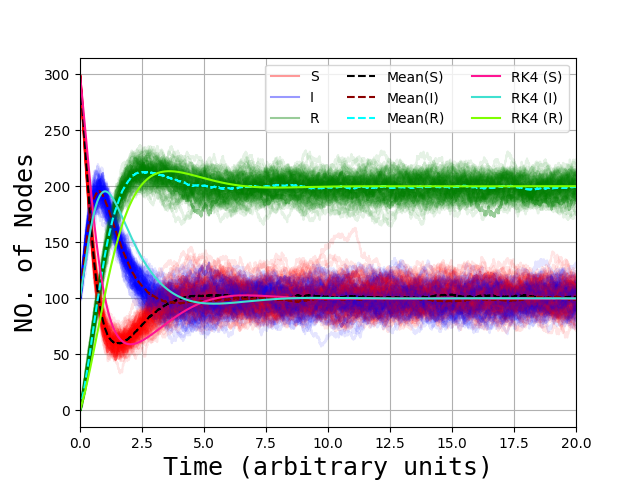
\includegraphics[width=1.1\linewidth]{Figures/OppgA_4_1_05.png}
			\caption{$\beta = 1$}
		\end{subfigure}
		\begin{subfigure}{0.49\linewidth}
			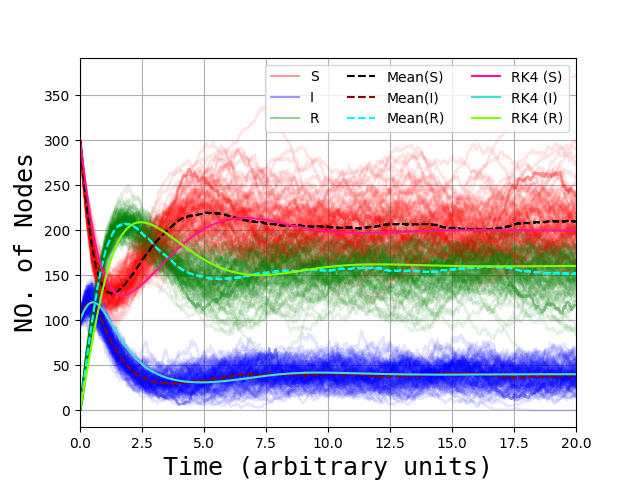
\includegraphics[width=1.1\linewidth]{Figures/OppgA_4_2_05.png}
			\caption{$\beta = 2$}
		\end{subfigure}
		\begin{subfigure}{0.49\linewidth}
			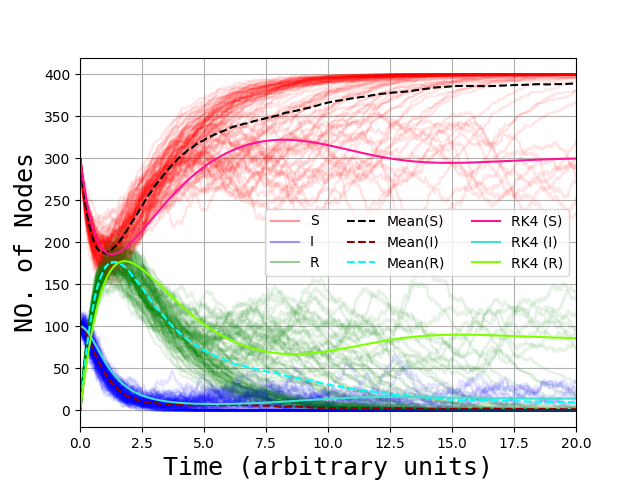
\includegraphics[width=1.1\linewidth]{Figures/OppgA_4_3_05.png}
			\caption{$\beta = 3$}
		\end{subfigure}
		\begin{subfigure}{0.49\linewidth}
		    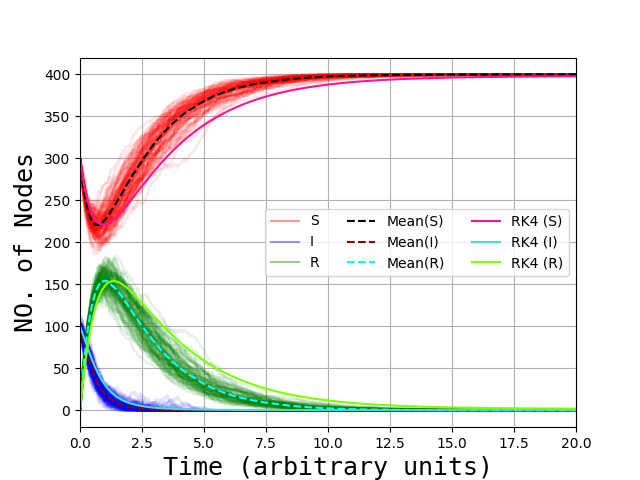
\includegraphics[width=1.1\linewidth]{Figures/OppgA_4_4_05.png}
			\caption{$\beta = 4$}
		\end{subfigure}
		\caption{Temporal development of the S, I and R populations, with different initial value for $\beta$, the rate of recovery. $\alpha = 4$ and $\gamma = 0.5$}
		\label{fig:1}
	\end{figure}
	
The four plots in Figure \ref{fig:1} shows the development of the populations of S, I and R with time with different values of $\beta$ for each plot. The values for $\alpha$ and $\gamma$ are held constant. For each plot, the Monte Carlo simulation has been run 100 times. These are the fine red, green and blue lines with varying degree of hue seen in the plots. This allows a deeper shade of color to be interpreted as statistically more common outcomes. The dashed lines show the expectation values at each point in time between all the simulations. The solid lines correspond to the Runge-Kutta solutions.

\begin{table}[H]
\centering	
\begin{tabular}{|c||c|c|c|c|}
\hline
\multicolumn{5}{|c|}{S}\\
\hline
$\beta$&1&2&3&4\\
\hline\hline
$S_\infty$& 100 & 200 & 300 & 400\\
\hline
RK4& 99.75 & 199.90 & 300.24& 397.80\\
\hline
MC& 101.94 & 207.51 & 380.68 & 399.98\\
\hline
\end{tabular}
\begin{tabular}{|c||c|c|c|c|}
\hline
\multicolumn{5}{|c|}{I}\\
\hline
$\beta$&1&2&3&4\\
\hline\hline
$I_\infty$& 100 & 40 & 14.28 & 0 \\
\hline
RK4& 100.08 & 40.07 & 14.06 & 0.21\\
\hline
MC& 98.21 & 37.22 & 1.98 & 0.0\\
\hline
\end{tabular}
\begin{tabular}{|c||c|c|c|c|}
\hline
\multicolumn{5}{|c|}{R}\\
\hline
$\beta$&1&2&3&4\\
\hline\hline
$R_\infty$& 200 & 160 & 85.71 & 0\\
\hline
RK4& 200.17 & 160.03 & 85.70 & 1.99\\
\hline
MC& 199.85 & 155.27 & 17.34 & 0.02\\
\hline
\end{tabular}
\caption{Expectation values for Monte Carlo simulations after equilibration. The final corresponding Runge-Kutta value, and the fraction of people in each population at equilibrium, for each value of $\beta$.}
\label{table:2}
\end{table}

Table \ref{table:2} shows the total number of agents occupying each compartment at equilibrium for each of the four different networks as computed by the expressions in \eqref{sirseq}. This is compared to the final value from the plots in Figure \ref{fig:1}, where "RK4" is the value obtained from the Runge-Kutta solver, and "MC" is the expectation value acquired across all 100 simulations. 



\begin{table}[H]
\centering
\begin{tabular}{|c||l|l||l|l||l|l|}
\hline
\multirow{2}{*}{$\beta$}
    & \multicolumn{2}{c||}{S}
        & \multicolumn{2}{|c||}{I}
            & \multicolumn{2}{|c|}{R} \\   \cline{2-7}
 & $\sigma$ & $\bar{x}$ & $\sigma$ & $\bar{x}$ & $\sigma$ & $\bar{x}$\\ \hline
 1&11.62&101.94&12.39&98.21&9.30&199.85 \\ \hline
 2&29.70&207.51&13.02&37.22&1.99&155.27 \\ \hline
 3&23.96&380.68&3.22&1.98&21.29&17.34 \\ \hline
 4&0.14&399.98&0.0&0.0&0.14&0.02 \\ \hline
\end{tabular}
\caption{Expectation values $\bar{x}$ and standard deviations $\sigma$ for the Monte Carlo simulations after equilibrium.}
\label{table:3}
\end{table}
Table \ref{table:3} shows the expectation values across 100 Monte Carlo simulations at equilibrium as well as the standard deviation, for varying values of $\beta$. 

%VITAL DYNAMICS
 \begin{figure}[H]
		\centering
		\begin{subfigure}{0.49\linewidth}
			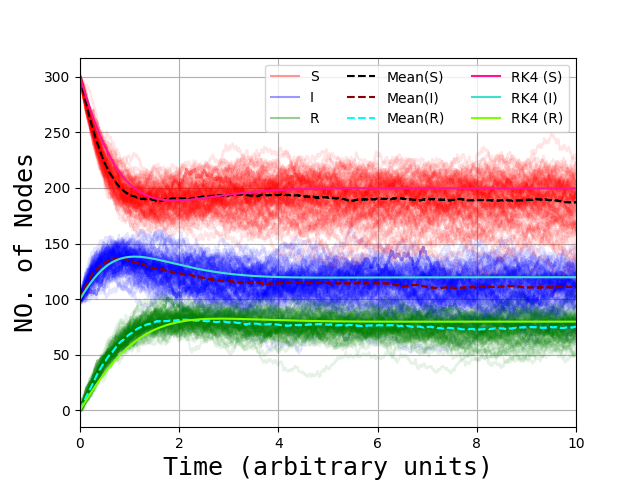
\includegraphics[width=1.1\linewidth]{Figures/OppgB_1_0_1.png}
			\caption{$\alpha = 4$, $\beta = 1$, $\gamma=0.5$, $\mu=1$, $\mu^*=0$, $\epsilon=1$}
		\end{subfigure}
		\begin{subfigure}{0.49\linewidth}
			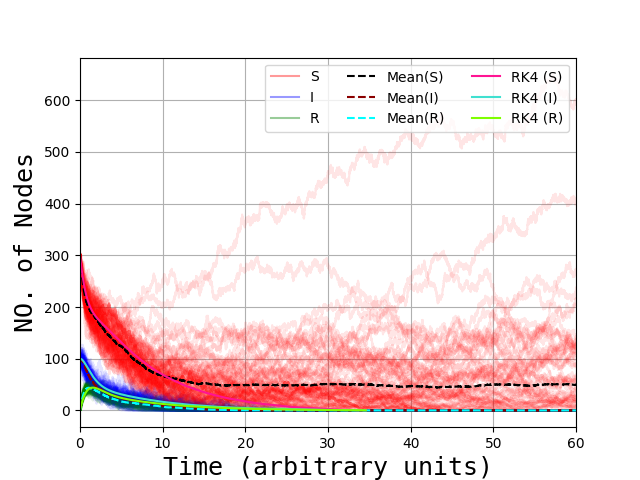
\includegraphics[width=1.1\linewidth]{Figures/OppgB_1_1_1.png}
			\caption{$\alpha = 4$, $\beta = 1$, $\gamma=0.5$, $\mu=1$, $\mu^*=1$, $\epsilon=1$}
		\end{subfigure}
		\begin{subfigure}{0.49\linewidth}
			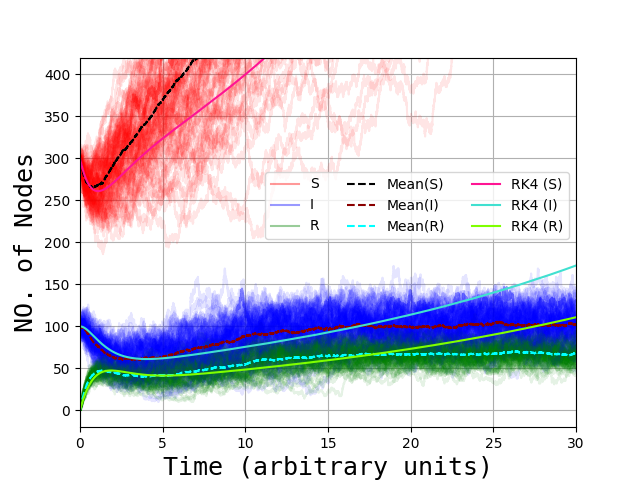
\includegraphics[width=1.1\linewidth]{Figures/OppgB_1_1_12.png}
			\caption{$\alpha = 4$, $\beta = 1$, $\gamma=0.5$, $\mu=1$, $\mu^*=1$, $\epsilon=1.2$}
		\end{subfigure}
		\begin{subfigure}{0.49\linewidth}
		    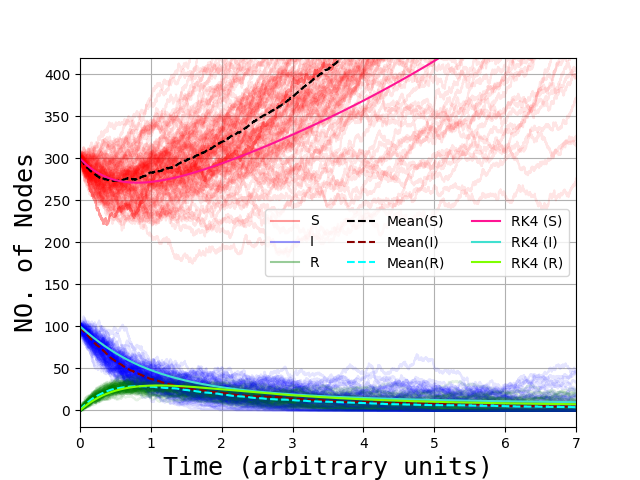
\includegraphics[width=1.1\linewidth]{Figures/OppgB_1_2_12.png}
			\caption{$\alpha = 4$, $\beta = 1$, $\gamma=0.5$, $\mu=1$, $\mu^*=2$, $\epsilon=1.2$}
		\end{subfigure}
		\caption{Temporal development of the S, I and R populations, with vital dynamics modelled.}
		\label{fig:vitaldynamics}
	\end{figure}
	
Figure \ref{fig:vitaldynamics} have the SIR-models with vital dynamics enabled. The variables $\mu$, $\mu^*$ and $\epsilon$ govern the conditions respectively for death from natural causes, death from infection, and the birth rate.

%SEASONAL VARIATION
 \begin{figure}[H]
		\centering
		\begin{subfigure}{0.49\linewidth}
			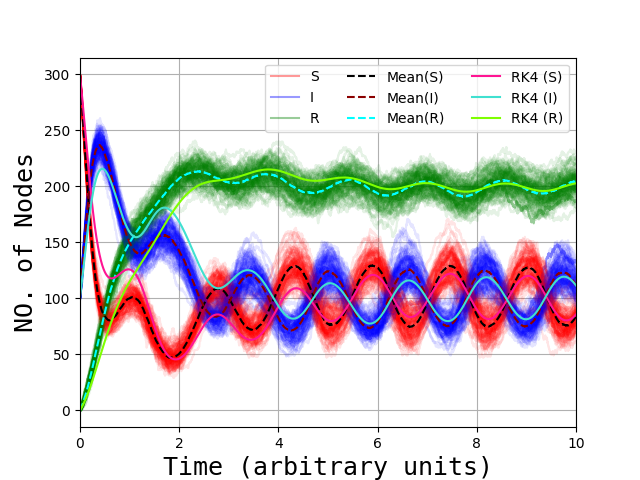
\includegraphics[width=1.1\linewidth]{Figures/OppgC_4_4.png}
			\caption{$\alpha_0 = 4$, $A = 4$, $\omega = 4$}
		\end{subfigure}
		\begin{subfigure}{0.49\linewidth}
			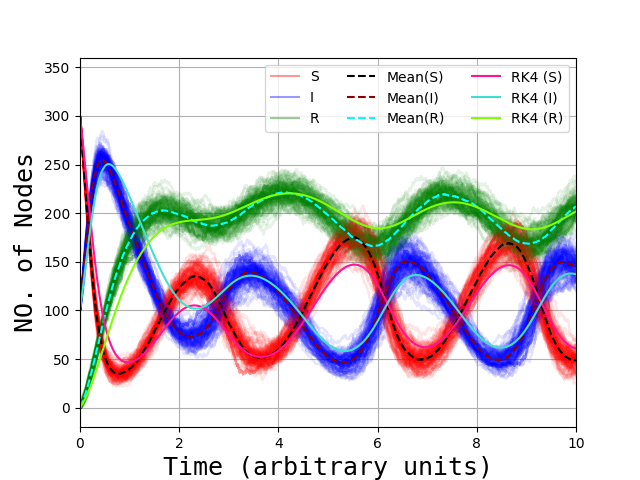
\includegraphics[width=1.1\linewidth]{Figures/OppgC_4_2.png}
			\caption{$\alpha_0 = 4$, $A = 4$, $\omega = 2$}
		\end{subfigure}
		\begin{subfigure}{0.49\linewidth}
			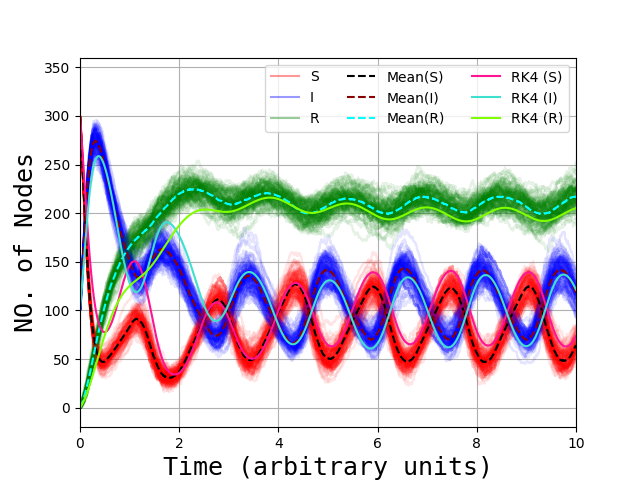
\includegraphics[width=1.1\linewidth]{Figures/OppgC_8_4.png}
			\caption{$\alpha_0 = 4$, $A = 8$, $\omega = 4$}
		\end{subfigure}
		\begin{subfigure}{0.49\linewidth}
		    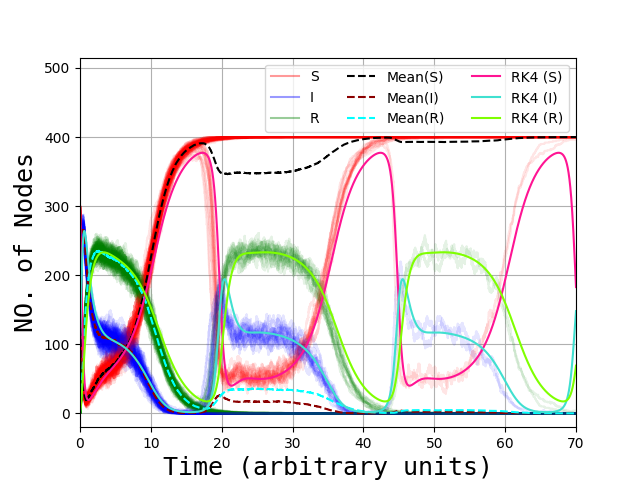
\includegraphics[width=1.1\linewidth]{Figures/OppgC_4_025.png}
			\caption{$\alpha_0 = 4$, $A = 4$, $\omega = 0.25$}
		\end{subfigure}
		\caption{Development with seasonal variation enabled. Different values for $A$ and $\omega$ have been used.}
		\label{fig:seasonalvar}
	\end{figure}
Figure \ref{fig:seasonalvar} displays four different simulations of the spread of disease in a network where we enable seasonal variation in the rate of infection, $\alpha(t)$. 
%Vaccination
 \begin{figure}[H]
		\centering
		\begin{subfigure}{0.49\linewidth}
			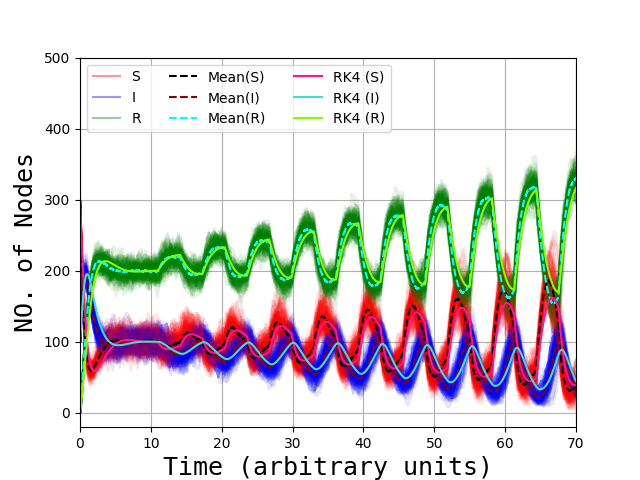
\includegraphics[width=1.1\linewidth]{Figures/Vax_Pulse2t_ckonst_4_1_05.png}
			\caption{Pulse vaccination, constant $\gamma$}
		\end{subfigure}
		\begin{subfigure}{0.49\linewidth}
			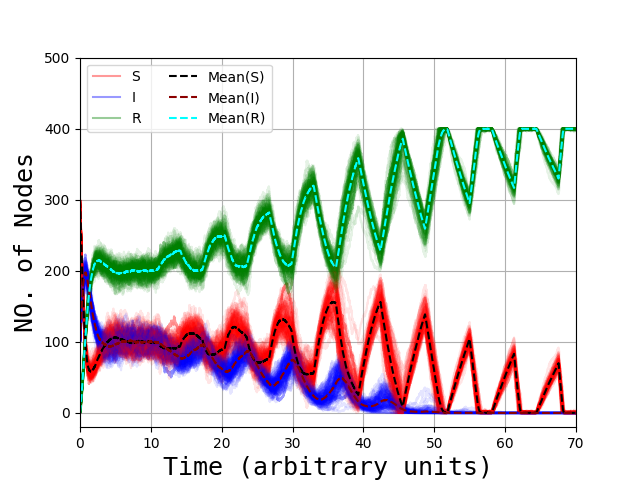
\includegraphics[width=1.1\linewidth]{Figures/Vax_Pulse2t_cvar_4_1_05.png}
			\caption{Pulse vaccination, variable $\gamma$}
		\end{subfigure}
		\begin{subfigure}{0.49\linewidth}
			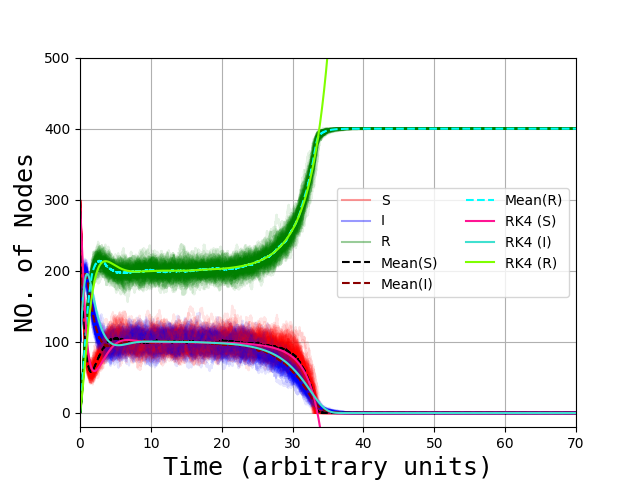
\includegraphics[width=1.1\linewidth]{Figures/Vax_expt_15x03_ckonst_4_1_05.png}
			\caption{Exponential vaccination, constant $\gamma$}
		\end{subfigure}
		\begin{subfigure}{0.49\linewidth}
		    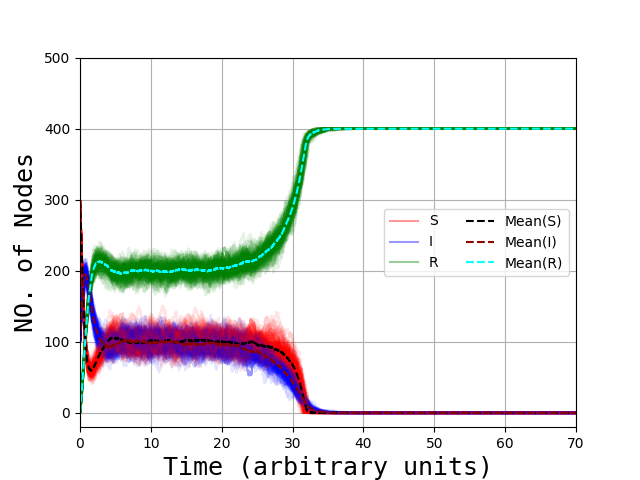
\includegraphics[width=1.1\linewidth]{Figures/Vax_expt_15x03_cvar_4_1_05.png}
			\caption{Exponential vaccination, variable $\gamma$}
		\end{subfigure}
		\caption{Development with vaccination with $\alpha = 4$, $\beta = 1$, $\gamma=0.5$ after time 10 for a and b and after time 15 for c and d}
		\label{fig:vaccinationvar}
	\end{figure}

Figure \ref{fig:vaccinationvar} displays the results obtained for simulations in which different vaccination programs are initiated after a given time $t$. In Figure \ref{fig:vaccinationvar} (b) we have implemented a function which decreases the rate of recovery $\gamma$ as discussed in Section \ref{section:vacfunc}, and the same was done in Figure \ref{section:vacfunc}. In these plots the ODE solutions are not included as the variable rate of recovery was never implemented for this solver. 


	\section{Discussion}
%Oppgave 4d
Figures \ref{econvergence} and \ref{mconvergence} show a clear trend in equilibration times for both the mean energy and mean magnetization for ordered and disordered systems. In both cases, for the 'cold' temperature $k_B T = 1\ J$, the systems initialized with ordered (ground state) spin configurations are already at equilibrium. Initializing the systems with ordered configurations (all up/all down) leads to only one possible energy change when proposing new configurations, being $\Delta E = 8J$. Hence, in all trials, the energy is never smaller than zero and so we do not immediately accept proposed configurational transitions. The algorithm will instead in each trial test random numbers against the distribution function, which leads to very low acceptance ratios. The ground state initialization for cold systems is therefore very stable. For an initially disordered configuration, we see that the system still quickly reaches equilibrium. An initially disordered configurations leads to more possible energy changes when flipping single spin sites, which dramatically increases the acceptance ratio in each trial. Still, the initial configuration is significantly different from the steady state configuration, which consequentially requires the algorithm to propose many different configurations before reaching the steady state configuration. Once steady state has been achieved, the situation is similar as for the initially ordered system - the acceptance ratio becomes very low. 

The situation is a bit different for the 'hotter' temperature $k_B T = 2.4\ J$. As can be seen from the plots, the system never completely stabilizes for the number of MCS used in these specific calculations. We here present the obtained data for $10^4$ cycles only as this data clearly displays the oscillatory behaviour as the system converges towards a steady state.  Therefore, an arbitrary degree of accuracy has to be chosen for what is considered an equilibrium state. For the mean energy in the right side of Figure \ref{econvergence}, it seems that after 3500 MCS, the two systems are fairly stable and seems to be oscillating around the same value. The same number of MCS can be accepted as the equilibration period for the mean magnetization in the right of Figure \ref{mconvergence}, although the oscillations around the equilibrium value are larger in magnitude.\\


As we may see in Figure \ref{fig:expvals}, the solutions for $\langle E \rangle$ and $\langle |M| \rangle$ for different lattice sizes are well behaved across the entire temperature interval. The solutions for $C_V$ and $\mathcal{X}$ are fairly well behaved for smaller lattices like the "40x40" and "60x60" system. For larger lattices, however, like the "80x80" and "100x100" considered here, the solutions deviate from the same "smooth" evolution towards the critical temperature from the very beginning of the simulation. We suspect that this has to do with a numerical phenomenon known as \textit{critical slowing down} of the Metropolis Algorithm \cite{walter}, \cite{carlon},\cite{gould}. To better grasp the idea of this concept, consider the figure below

\begin{figure}[H]
    \centering
    \includegraphics[width = \linewidth]{Figure/magdomains.png}
    \caption{Plot of magnetic domains in a 100x100 spin lattice at different temperatures $k_B T = 1.0 J$ (left), $k_B T \sim T_C$ (middle) and $k_B T = 2.6 J$ (right). The red color represents the spin down attribute at a lattice site, and the black color represents the spin up attributes. }
    \label{fig:domains}
\end{figure}

Figure \ref{fig:domains} illustrates the formation of magnetic domains in a spin lattice, and how such clusters of aligned spins form accordingly with temperature. As we presented in Figure \ref{fig:expvals}, the absolute magnetization of the spin lattice incrementally evolves towards zero - id est a state in which there are equal amounts of spin up and spin down sites. The rightmost figure in \ref{fig:domains} indicates that the system follows such an evolution, as the spin clusters become more evenly distributed in size\footnote{This behaviour would have been more easily recognized had we simulated the system over a larger temperature interval such that the final temperature had been much larger than the initial temperature.}. Nevertheless, the most important feature of this spin cluster model in this context is that around the critical temperature, the spin lattice consists of many, unevenly distributed domains of aligned spins. When performing random sampling at this temperature, the single spin flip dynamic we devise in this algorithm leads to an exceptionally low acceptance rate. Consider, like before the 2D Ising model in which a spin center has four nearest neighbors. At $T_C$, such spin centers have four nearest neighbors which are all aligned with the spin center, with the exception of spin centers located at the boundary of two spin domains. Flipping the spin center leads to a change in the local energy contribution of size $\Delta E = 8J$ as we discussed in Section 3.2, committing to an acceptance rate $A(i \to j) = \exp(-8\beta_C) \approx 0.03$ for $\beta_C = 1/(k_B T_C)$ where $T_C$ holds the approximate value $T_C \approx 2.269$. Worse still, given that a local spin center in a spin cluster is flipped by chance, sampling this local spin configuration in a later Monte Carlo Sweep guarantees that the spin will be flipped back as this proposed transition carries a local energy change $\Delta E = -8J < 0$, which the algorithm accepts without exception. The odds of transitioning between many states in configuration space and sampling a decent amount of significantly incoherent data are very much stacked against us at temperatures around $T_C$, all due to the critical slow down of the Metropolis algorithm stemming from the formation of aligned spin clusters.\\

As we can see, sweeping through the lattice, each time seeding a random lattice site, the spin cluster formation manifests strong correlation between two proposed configurations. The critical slowing down of the Metropolis algorithm is largely dictated by the \textit{correlation time}. The correlation time $\tau$, in units of Monte Carlo Sweeps per lattice point, is an approximate measure of how many iterations that are necessary for two different configurations to be significantly incoherent. For sufficiently large lattices with single spin flip dynamics, the correlation time is given by

\[
\tau \sim \mathcal{L}^{z_c}
\]
where $\mathcal{L}$ is the size of the lattice, and $z_c$ is the \textit{critical dynamical exponent} which Nightingale and Blöte obtained as $z_c = 2.1665(12)$ for single spin flip dynamics in the square spin lattice case \cite{nightingale}. The correlation time is a much more accurate representation of the actual equilibration time $t$, an important quantity which we crudely have determined by visual inspection in this project. Inspecting $\tau$, we see that the correlation time between a two states is close to ten thousand Monte Carlo sweeps \textit{per lattice site}, leading up to the fact that a total of one hundred million Monte Carlo sweeps would suffice for random sampling of incoherent states, which in turn would lead to significantly more accurate data. In light of the time it took to run the program using a total of ten million cycles for the 80x80 and 100x100 systems for our rather high temperature resolution, amping up the total number of Monte Carlo cycles is a study prospect for our future selves. In our research we have found that so called 'cluster algorithms' established by Wolff, as well as Swendsen and Wang \cite{walter} solve this issue by flipping entire clusters of aligned spins rather than singular spins.\\

Although the data obtained for the larger systems in this study is far less accurate than desired, these solutions too commit a clear indication of where the system undergoes a phase transition, which was helpful in the numerical extraction of the critical temperature. By determining the temperatures for which each curve describing either $\mathcal{X}$ and $C_V$ have a clear maximum value, the true value of the critical temperature $T_C$ may be found through the relationship \eqref{critical2} described in Section \ref{sectioncritical}. These temperatures are given in Table \ref{tab:Tc_susc} and a plot of the data alongside with the the associated linear regression is shown in Figure \ref{fig:tcritical}. We found the critical temperature for an infinite lattice to be $2.289$, whereas the analytical value obtained by Onsager is $\approx 2.269$. This is an error of just $0.8$\%, and therefore a very good approximation. By running the program for larger lattice sizes ($\mathcal{L} > 100$), and also taking the longer correlation times into consideration such that the data displays singular global maxima, an even better approximation could be made.
	\section{Conclusion}
The Metropolis-Hastings algorithm proves to be an effective tool for modelling the Ising model in two dimensions. We've managed to produce values for mean energy and magnetization with relative errors in the order of $10^{-5}$ compared to analytical values for the same system. Because of propagation of statistical error, the values gotten for mean heat capacity and susceptibility are not quite as accurate when compared to analytical values. For 20x20 lattices, we see very clearly how the system has an equilibration time, before it reaches a steady state. This fact is confirmed when we consider the amount of accepted states as a function of Monte Carlo cycles. One of the main goals has been to find the critical temperature where a second-order phase transition happens. By modelling increasingly larger lattices, we can see clear indications of the temperature where a phase transition occurs. Using the data from these large lattices, we approximate the critical temperature for an infinitely large lattice. The critical temperature approximated this way differs from the analytical value by only 0.8\%, which is a tremendously good result, and a proof of just how good the Metropolis-Hastings algorithm is when applied to the Ising model. However, as we have encountered frequently during this project, the Metropolis-Hastings algorithm is quite computationally heavy. For lattices of size 100x100, the program had to run for over 20 hours in some cases, even using parallelized code running on 4 CPU cores. For future projects, code should be tested extensively to make sure that it performs faultlessly, and then be run on a more powerful system, like the BigFacet\footnote{\url{https://www.mn.uio.no/fysikk/english/people/adm/almarin/ccse-servers.html}} server. In addition to this, we have also for larger lattices encountered critical slowing down at the critical temperature, a numerical flaw which occurs due to the formation of aligned spin domains, and the corresponding correlation time committed by the single spin flip dynamics.
	
	\newpage
	\addcontentsline{toc}{section}{References}
	\begin{thebibliography}{5}
        \bibitem{statphys}
        M. Plischke and B. Bergersen, \textit{Equilibrium State Physics}, World Scientific, chapters 5 and 6
        \bibitem{nightingale}
        Nightingale, M. P. and Bl\"ote, H. W. J. (1996), \textit{Dynamic Exponent of the Two-Dimensional Ising Model and Monte Carlo Computation of the Subdominant Eigenvalue of the Stochastic Matrix}. Phys. Rev. Lett. 76, 24, pp. 4548-4551
        \bibitem{walter}
        J.-C. Water and G.T. Barkema, \textit{An introduction to Monte Carlo methods}. PDF, 6-8. \\
        \url{https://arxiv.org/pdf/1404.0209.pdf}
        \bibitem{carlon}
        Carlon, E. (2013), \textit{Advanced Monte Carlo Methods.} PDF, 15-16\\
        \url{http://itf.fys.kuleuven.be/~enrico/Teaching/monte_carlo_2012.pdf}
        \bibitem{gould}
        Harvey, G. and Tobochnik, J. (1989), \textit{Overcoming Critical Slowing Down}. PDF, 1-3.\\
        \url{https://aip.scitation.org/doi/pdf/10.1063/1.4822858}
	\end{thebibliography}
	
\end{document} 